% Chapter Template 
% cSpell: words Mininet prototipado parencite enrutamiento includegraphics veth  mininetonf cellcolor Nicira vswitchd interconectar multicapa datapath ovsflow resizebox flowtable netlink OVSDB dpctl ofctl vsctl rowcolor mininetovs
 
\chapter{Análisis de las tecnologías} % Main chapter title

\label{Chapter3} % Change X to a consecutive number; for referencing this chapter elsewhere, use \ref{ChapterX}

Teniendo en cuenta los conceptos revisados en el capítulo anterior, en este se estudiarán las herramientas que permitirán la realización del proyecto. 

En la primera sección, se realizará un análisis del dispositivo utilizado, un \textit{muxponder} óptico coherente de 40GB desarrollado por la institución donde se realizó el proyecto.

Luego, en la segunda sección se examinarán las herramientas de software involucradas. La misma se encuentra dividida en dos partes; la primera detalla el funcionamiento del controlador \textit{SDN} utilizado, \textit{ONOS}; la segunda refiere al estudio de dos agentes \textit{NETCONF}: Sysrepo y Yuma123.


%----------------------------------------------------------------------------------------
%	SECTION 1
%----------------------------------------------------------------------------------------

\section{Herramientas de Hardware}

Para cumplir con el objetivo del proyecto, será de suma importancia conocer las bondades y las limitaciones del equipo con el que se cuenta. Así, esta sección comprende el estudio de uno de los dispositivos mencionados en el capítulo anterior, un \textit{muxponder}. Concretamente, se analizarán aspectos técnicos relacionados tanto al hardware como al software de un \textit{muxponder} de 40GB. El interés del análisis resulta en que es en este dispositivo en donde se integrará el protocolo de gestión \textit{NETCONF}.

\subsection{\textit{Muxponder} 40GB}

El muxponder con el que se cuenta es capaz de realizar una transmisión óptica de 40GB/s sobre una señal de línea \textit{OTU3}. La misma es lograda cumpliendo el estándar \textit{ITU-T G.709} \parencite{itu7}, utilizando una modulación coherente \textit{DP-QPSK} o \textit{DP-DQPSK}.
Dispone de cuatro clientes ópticos asíncronos totalmente independientes de 10GB/s cada uno, a través de módulos ópticos  \textit{XFP} removibles. Las longitudes de ondas soportadas para los clientes son 850/1310/1550 nm y admite los tipos de cliente \textit{10GB Ethernet LAN/WAN, OTU2} y \textit{OTU2e}.
\\

Además, incorpora el mecanismo de corrección de errores \textit{FEC} para todas las señales, tanto para clientes como para línea. Mediante el mismo, el \textit{muxponder} es capaz de realizar correcciones sin necesidad de retransmitir la información.
\\

En términos de potencia, alcanza típicamente los 93 Watts. También, el dispositivo puede alcanzar una distancia de hasta 2000Km.
\\

Las interfaces de conexión soportadas para realizar configuración y monitoreo en el dispositivo son: 
\begin{itemize}
	\item 2 puertos \textit{Ethernet}.
	\item 1 puerto serial \textit{RS232}.
	\item 1 puerto \textit{USB} 2.0.
\end{itemize}

En la figura \ref{fig:mux40} se puede observar en el panel frontal del equipo con las diferentes interfaces mencionadas anteriormente.


\begin{figure}[H]
	\centering
	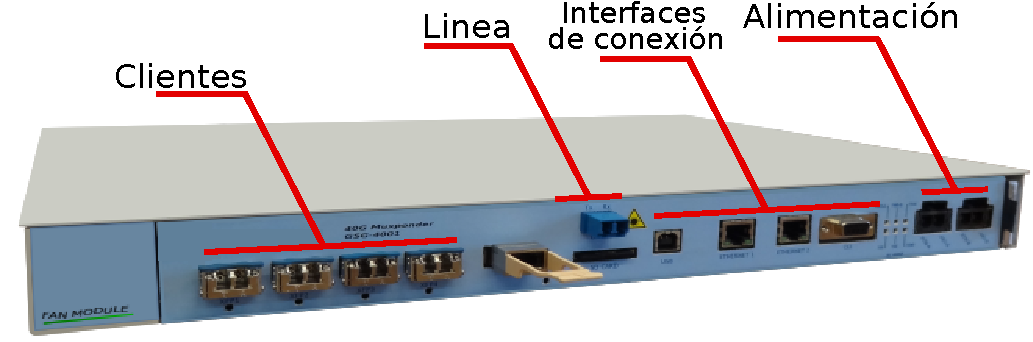
\includegraphics[scale=0.7]{Figures/mux40.pdf}
	\caption{Vista del panel frontal del \textit{muxponder} de 40GB utilizado.}
	\label{fig:mux40}
  \end{figure}

  Por otra parte, el \textit{muxponder} de 40GB integra un total de 128MB de memoria \textit{RAM} y 512MB de almacenamiento, con capacidad de extender esta última mediante una tarjeta \textit{SD}. Además, cuenta con un sistema operativo Linux \textit{'Buildroot'}, el cual ocupa gran parte de estos recursos mencionados, dejando libre para las aplicaciones de usuario un total de 100MB de \textit{RAM} y 270MB de almacenamiento.

El hecho de que presente dicho sistema operativo resulta en una ventaja por varios motivos, en primer lugar porque el mismo es un entorno conocido por el alumno, donde además podrán ejecutarse en él la mayoría de las aplicaciones \textit{UNIX} típicas. En segundo lugar, el sistema operativo integra librerías y herramientas que facilitarán el desarrollo del proyecto, como por ejemplo la librería \textit{SSH}, necesaria por el protocolo \textit{NETCONF}.
\\

Por último, el procesador que incorpora es un \textit{NIOS II} de primera generación fabricado por \textit{Intel} \parencite{intelaltera}. El mismo funciona a 125 Mhz y se encuentra integrado en una \textit{FPGA}. Es importante destacar que la arquitectura de este procesador no es una arquitectura típica de una máquina de propósito general (por ejemplo \texttt{x86\_64}), por lo tanto, las distintas aplicaciones que se ejecuten en esta plataforma deberán estar compiladas específicamente para la arquitectura \textit{NIOS}. 

Además, debido a las capacidades de la memoria primaria y secundaria del equipo, resulta imposible realizar la compilación de las aplicaciones sobre el mismo. Por lo tanto, se deberá realizar lo que se conoce como compilación cruzada, que consiste en preparar un sistema huésped (donde generalmente dicho sistema cuenta con mayores recursos y capacidades) para generar todos los binarios y librerías que requiere el dispositivo objetivo donde finalmente se ejecutarán las aplicaciones.

\newpage

\subsection{Componentes del \textit{muxponder}}

Los componentes más significativos del dispositivo se listan a continuación:

\begin{itemize}
	\item Módulo de 40GB.
	\item Los 4 puertos clientes (XFP).
	\item Unidad de ventilación.
	\item Chip cortina.
	\item Unidad de alimentación.
	\item Interfaces de control.
	\item \textit{FPGA}, con el procesador \textit{NIOS II} instanciado.
\end{itemize}


Además, se presenta en la figura \ref{fig:diagramabloque} un diagrama en bloques del \textit{muxponder}, donde se pueden observar los principales componentes que conforman el mismo.

\begin{figure}[H]
	\centering
	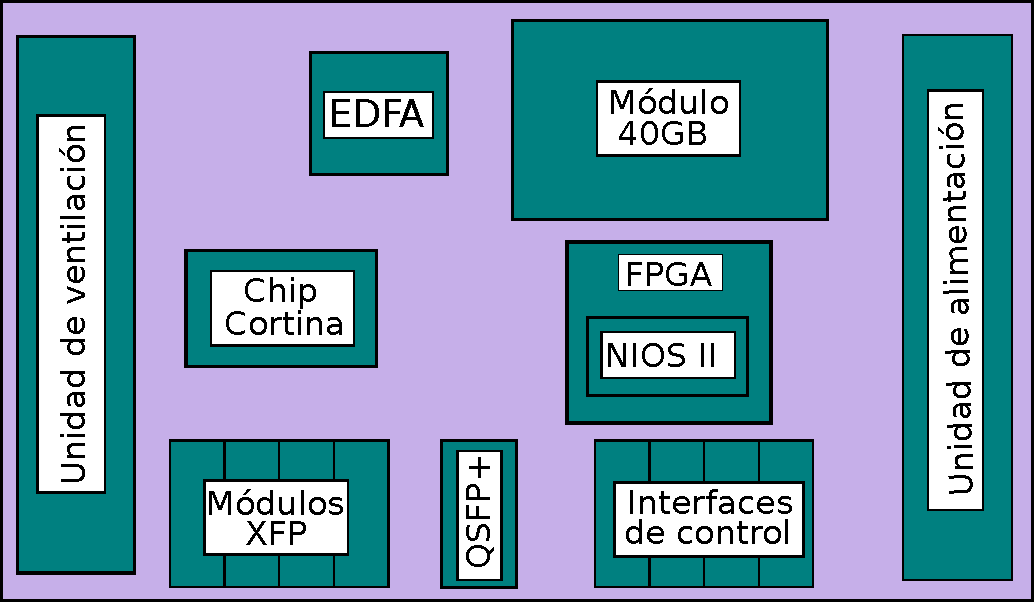
\includegraphics[scale=0.60]{Figures/diagramabloquesmxp.pdf}
	\caption{Diagrama en bloques del \textit{muxponder} de 40GB.}
	\label{fig:diagramabloque}
  \end{figure}

Por otra parte, una vista de la circuitería del equipo se puede observar en la figura \ref{fig:diagramabloquemxp}.

\begin{figure}[H]
	\centering
	\includegraphics[scale=0.060]{Figures/bloquemxpfisico-min.pdf}
	\caption{Vista de la circuitería del \textit{muxponder} de 40GB.}
	\label{fig:diagramabloquemxp}
  \end{figure}

\subsection{Aplicaciones integradas en el dispositivo}

Será importante explicar la utilidad de dos binarios que incorporan los \textit{muxponders} de 40GB: 'monitor' y 'muxponder'. 

\begin{itemize}
	\item \textbf{'monitor'}: aplicación que permite mostrar información del dispositivo a través de la \textit{CLI}. Con el fin de agrupar y ordenar los datos relacionados, los mismos se encuentran divididos en secciones. Por ejemplo, se tiene una sección dedicada a mostrar la temperatura de los diferentes módulos, las alarmas relacionadas a la transmisión y recepción, otra sección referida a la presencia de los módulos XFP del equipo, entre otros. De esta forma, el administrador podría conocer el estado del dispositivo ejecutando dicha aplicación y observando la salida producida en pantalla.
	
	Por otra parte, el equipo utiliza el método de comunicación entre procesos llamado memoria compartida. El mismo consiste en una región de memoria donde se permite que otras aplicaciones puedan, por ejemplo, leer información. Así, la aplicación 'monitor' también es la encargada de actualizar en memoria compartida los valores de todos los datos a monitorear, permitiendo que otras aplicaciones puedan leer y acceder a dicha información.
	
	A continuación, se muestra en la figura \ref{fig:monitor} una porción de la salida en pantalla producida por la aplicación 'monitor'. En ella se puede observar la sección relacionada a los módulos XFP del \textit{muxponder}.
	
	\begin{figure}[H]
		\centering
		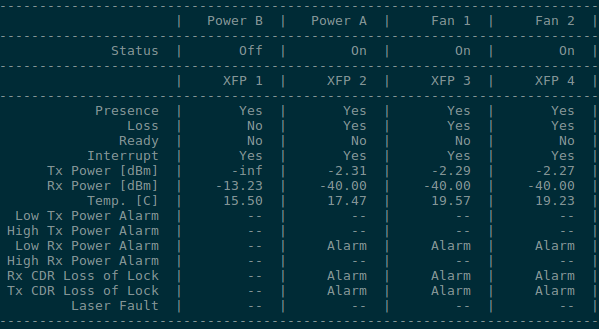
\includegraphics[scale=0.77]{Figures/monitorapp.png}
		\caption{Sección XFP de la aplicación ’monitor’.}
		\label{fig:monitor}
	  \end{figure}

	\item \textbf{'muxponder'}: Por otra parte, la aplicación 'muxponder' es utilizada por el administrador para poder configurar el dispositivo mediante ciertos parámetros que son especificados haciendo uso de la \textit{CLI} del equipo. Por ejemplo, con esta aplicación el administrador podría cambiar la configuración de un \textit{muxponder} que tiene un tipo de tráfico $otu2$ por un tipo de tráfico $xge$ a través de la CLI, tal como se muestra en la figura \ref{fig:mxpapp}.

	\begin{figure}[H]
	  \centering
	  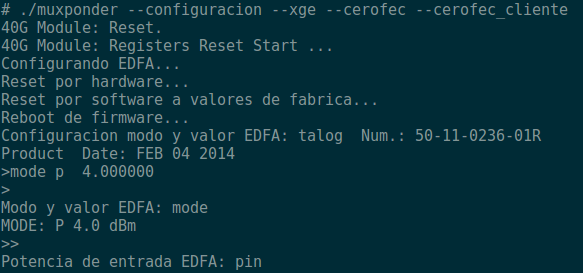
\includegraphics[scale=0.63]{Figures/muxponderapp.png}
	  \caption{Configuración mediante la aplicación ’\textit{muxponder}’.}
	  \label{fig:mxpapp}
	\end{figure}
\end{itemize}



  

%----------------------------------------------------------------------------------------
%	SECTION 2
%----------------------------------------------------------------------------------------



\section{Herramientas de Software}

Además del estudio del hardware utilizado, resulta de interés realizar un análisis de los componentes de software que conforman el proyecto. Para ello, la primer parte de esta sección estará dedicada a estudiar el controlador \textit{SDN} empleado, mientras que en la segunda parte se analizarán dos agentes \textit{NETCONF} disponibles de código abierto.

\subsection{Controlador \textit{ONOS}}
El controlador \textit{ONOS}, desarrollado y mantenido por la \textit{ONF} \parencite{onff}, es uno de los controladores abiertos más comunes en la industria, donde destacan miembros como Google, Intel, \texttt{AT\&T}, Samsung, entre una numerosa lista \parencite{onffmembers}. Está diseñado específicamente para los proveedores de servicios, donde sus principales objetivos son la escalabilidad y el alto rendimiento \parencite{onffwhite}.

Las licencias compatibles con \textit{ONOS} son \textit{Apache} 2.0, \textit{MIT} y \textit{BSD} \parencite{onfflic}. El hecho de que sea un proyecto \textit{open-source}, supone ventajas como ser interoperabilidad, personalización, flexibilidad e independencia del fabricante. 

Antes de detallar cómo funciona y realizar un análisis de su arquitectura, es importante explicar el problema que enfrentan los controladores \textit{SDN} para poder entender las ventajas que supone el uso de \textit{ONOS} frente a otros controladores. 
\\

Debido al crecimiento del consumo de tráfico en las redes y la demanda del ancho de banda en alza, es necesario para los proveedores de servicio que el rendimiento y la escalabilidad de sus redes no se vean afectadas por estos motivos. De este modo, los controladores \textit{SDN} deben poseer tres atributos claves: escalabilidad, rendimiento y alta disponibilidad \parencite{sdnproblema}.

\begin{itemize}
	\item \textbf{Escalabilidad}: como se explicó en el capítulo anterior, \textit{SDN} introduce una autoridad de control centralizada. La misma, debe ser capaz de escalar de igual forma que las funcionalidades de la red, manteniendo su rendimiento.
	\item \textbf{Alta disponibilidad}: el plano de control que se encuentra centralizado en el controlador, juega ahora un papel crítico. Esto es así ya que si el mismo se encuentra sobrecargado o deja de estar disponible por alguna razón, la funcionalidad de la red se vería afectada. Por lo tanto, las diferentes soluciones \textit{SDN} deberán brindar disponibilidad ininterrumpida del controlador.
	\item \textbf{Rendimiento}: el controlador también tiene que ser capaz de proveer mecanismos para adaptarse dinámicamente ante las fluctuaciones en la carga del tráfico y la congestión de la red, evitando que el rendimiento del mismo se vea afectado. 
\end{itemize}

\subsubsection{Arquitectura del controlador}
Las características más importantes de la arquitectura presentada por \textit{ONOS} \parencite{onffwhite} se detallan a continuación:

\begin{itemize}
	\item \textbf{Núcleo distribuido}: la solución que propone \textit{ONOS} para proveer escalabilidad, alto rendimiento y disponibilidad, se basa en un núcleo distribuido por los diferentes nodos que conforman un \textit{cluster}, lo que implica la posibilidad de soportar enormes cantidades de dispositivos de red. Esto último es así ya que \textit{ONOS} permite la incorporación dinámica de nuevos nodos, con lo que la carga del controlador podría distribuirse entre ellos de forma adaptativa.
	
	La figura \ref{fig:onosdistribuido} ejemplifica dicha distribución. El hecho de agregar esta redundancia implica una mayor disponibilidad del controlador. A su vez, permite realizar un balanceo de carga, lo que se traduce en mayor rendimiento y escalabilidad.

	\begin{figure}[H]
		\centering
		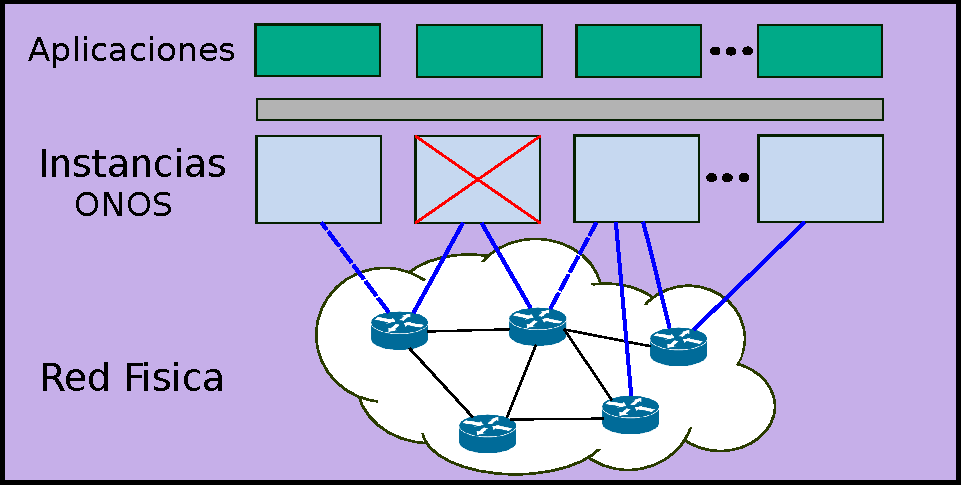
\includegraphics[scale=0.7]{Figures/onosarch.pdf}
		\caption{Arquitectura distribuida de \textit{ONOS}.}
		\label{fig:onosdistribuido}
	  \end{figure}


	\item \textbf{Abstracción \textit{Northbound}}: el plano aplicación explicado en el capítulo anterior, se comunica con \textit{ONOS} a través de una interfaz brindada por el controlador. El mismo, brinda a las aplicaciones gráficos y estadísticas de la red como así también aplicaciones basadas en \textit{intents} para facilitar el control, administración y configuración de los equipos.
	\item \textbf{Abstracción \textit{Southbound}}: de forma similar, el controlador ofrece una interfaz para comunicarse con el plano de datos. Cabe destacar que si bien \textit{ONOS} basa su funcionamiento en el protocolo \textit{OpenFlow}, también brinda soporte a otros como \textit{NETCONF}, \textit{REST}, \textit{SNMP}, etc, con el fin de mantener compatibilidad con dispositivos más antiguos.
	
	Una aproximación más detallada de la arquitectura que presenta \textit{ONOS} puede verse en la figura \ref{fig:onosarch}. En la misma, se observan las interfaces mencionadas anteriormente junto a una serie de componentes que pertenecen a la interfaz \textit{Southbound}. Estos componentes se analizarán más adelante. 

	\begin{figure}[H]
		\centering
		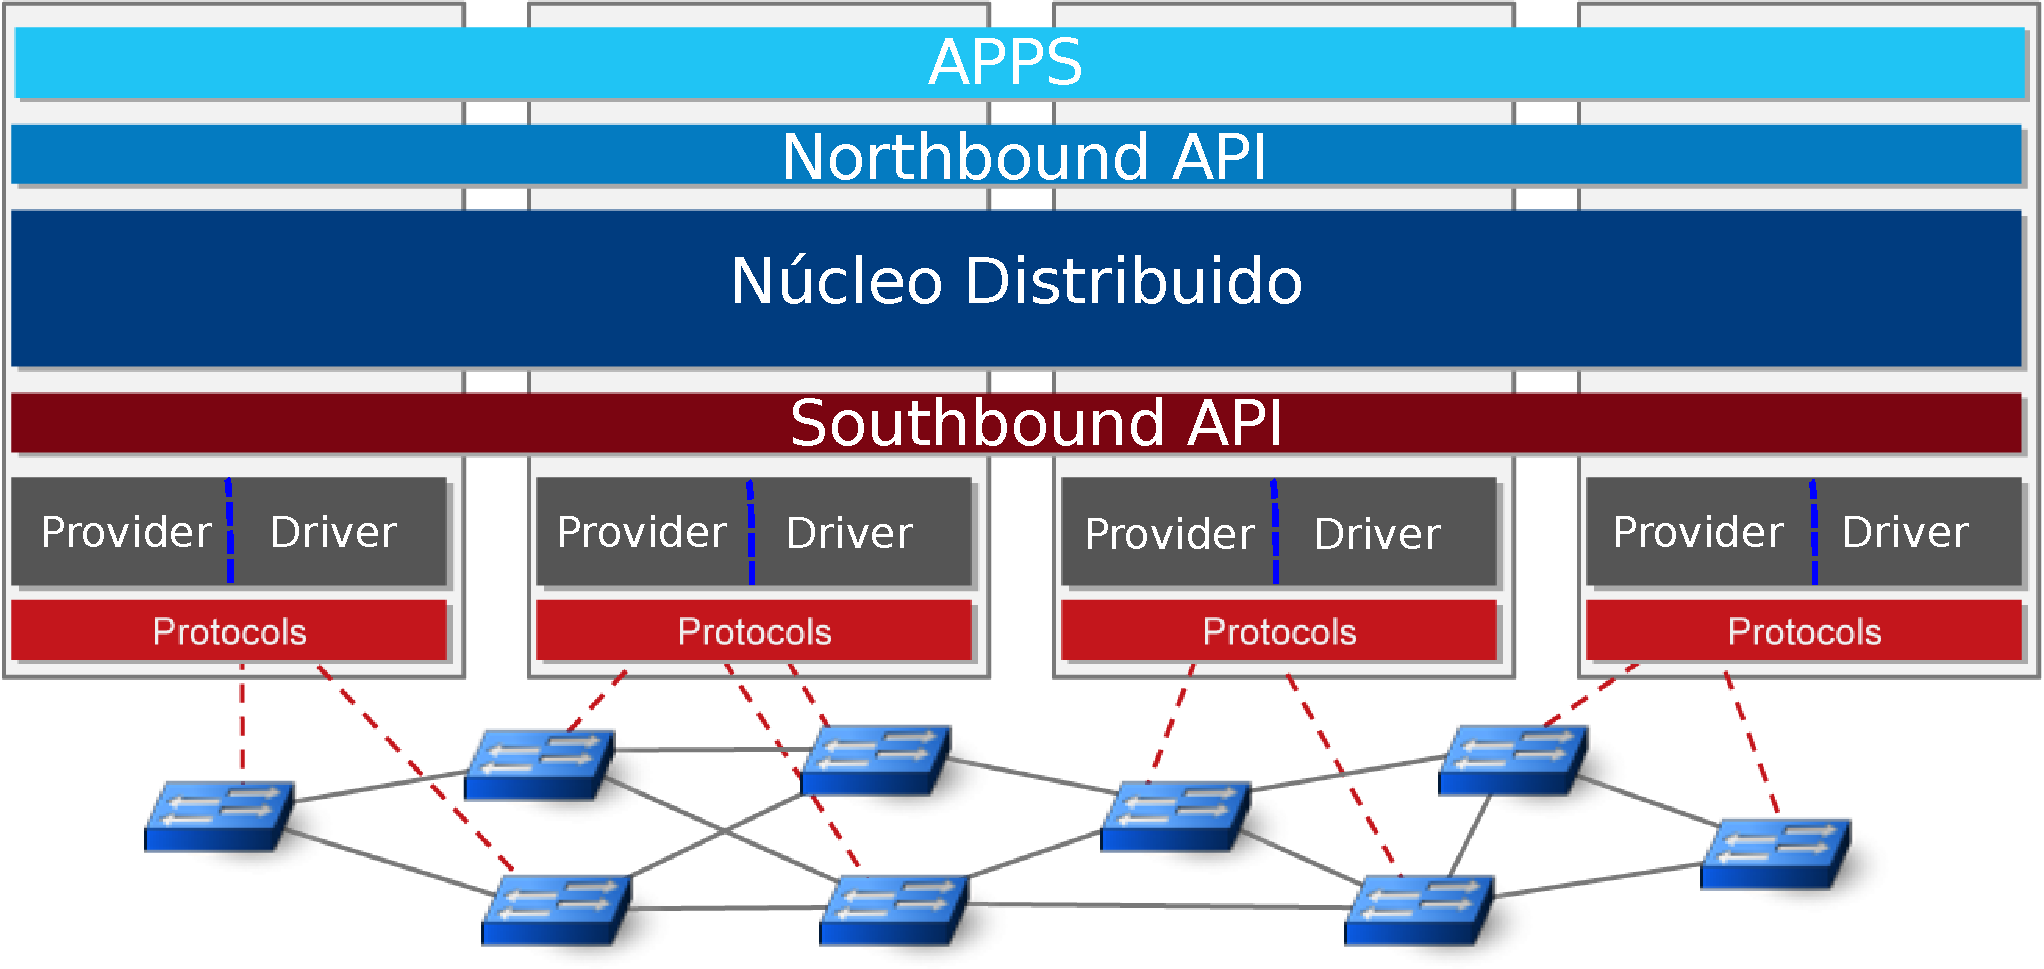
\includegraphics[scale=0.40]{Figures/corecompleto.pdf}
		\caption{Arquitectura completa del controlador \textit{ONOS}.}
		\label{fig:onosarch}
	  \end{figure}

	\item \textbf{Modularidad}: el controlador se encuentra desarrollado en \textit{Java}, y mediante el \textit{framework} OSGi obtiene las características de una arquitectura modular. De esta forma, se provee a los desarrolladores facilidad para brindar actualizaciones a sus aplicaciones, poder monitorearlas, realizar depuración y mantenimiento.  
\end{itemize}



  



  \subsubsection{Interfaz \textit{Southbound} en \textit{ONOS}}
  Tal como se explicó anteriormente, el objetivo del proyecto es gestionar la configuración de un \textit{muxponder} de 40GB a través del protocolo \textit{NETCONF}. 
  
  Para ello, será necesario explicar con más detalle la interfaz \textit{Southbound} de \textit{ONOS}. La misma se encuentra dividida en una serie de componentes que se detallan a continuación:

  \begin{itemize}
	\item \textbf{\textit{Providers}}: son aplicaciones independientes que residen en el núcleo de \textit{ONOS} y que pueden activarse o desactivarse dinámicamente en tiempo de ejecución. El propósito principal de esta capa es abstraer al \textit{core} las complejidades de los protocolos, brindando interfaces de las operaciones típicas y generales de los mismos. Un ejemplo de un \textit{provider} en \textit{ONOS} es el llamado \textit{'NetconfAlarmProvider'}, encargado de transformar cada notificación de los dispositivos en una alarma registrada en \textit{ONOS}.
	\item \textbf{\textit{Protocols}}: es la capa de más bajo nivel en la interfaz \textit{Southbound} y es la única que tiene contacto directo con los dispositivos conectados al controlador. Aquí se implementan los diferentes protocolos necesarios para la comunicación como ser \textit{NETCONF}, \textit{REST}, \textit{SNMP}, etc. Comúnmente en esta capa se utilizan librerías de terceros como \textit{openflowj, snmp4j, thrift}, entre otras.
	\item \textbf{\textit{Drivers}}: al igual que los \textit{providers}, los \textit{drivers} pueden cargarse dinámicamente al núcleo del controlador y proveen mecanismos para comunicarse con los diferentes dispositivos a través de algún protocolo. La diferencia principal con los \textit{providers}, es que aquí no se implementan generalidades de los protocolos, sino comportamientos específicos de los dispositivos. Además, sirve de interfaz entre las aplicaciones que se encuentran en la capa \textit{Northbound} y los diferentes equipos de red. El propósito principal de este subsistema es el de aislar el código específico del dispositivo, de tal manera de que el mismo no se extienda por el resto del núcleo de \textit{ONOS}. Dado que dicho código será necesario para cualquier futuro previsible, este subsistema proporciona medios para contenerlo y permitir que otros subsistemas (por ejemplo, la capa de aplicación) interactúen con él a través de abstracciones independientes del protocolo y del dispositivo. Por último, presenta una ventaja para los desarrolladores de hardware dado que al ser un componente modular, permite la herencia de funcionalidades de otros \textit{drivers} con el fin de compartir características con una familia de dispositivos en común.
\end{itemize}

La figura \ref{fig:onosarchsouth} esclarece la participación que tiene cada componente tanto con el \textit{core} como con el dispositivo.

\begin{figure}[H]
	\centering
	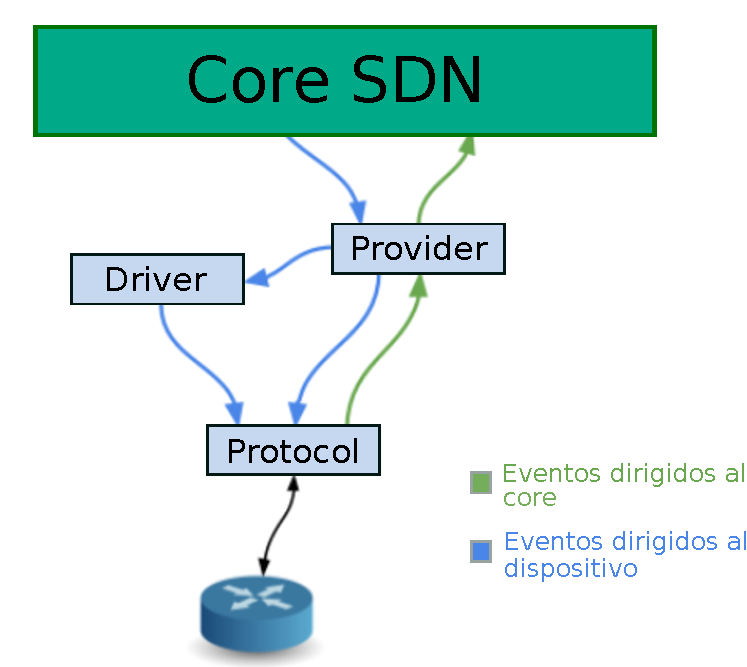
\includegraphics[scale=0.67]{Figures/southboundonos.pdf}
	\caption{Interfaz \textit{Southbound} en \textit{ONOS}.}
	\label{fig:onosarchsouth}
  \end{figure}

  \subsubsection{Justificación de la elección del controlador}

En la actualidad, existe una diversidad de controladores \textit{SDN}, como ser \textit{Ryu} (\textit{Python}), \textit{Floodlight} (\textit{Java}), \textit{POX} (\textit{Python}), e incluso implementaciones propietarias. 

Se destaca \textit{OpenDaylight} (\textit{Java}), un controlador abierto que soporta una gran lista de protocolos y que, según \parencite{book_SDN_a_c_a}, junto a \textit{ONOS} es uno de los controladores más utilizados en la industria.

La razón determinante por la cual se optó por \textit{ONOS} como controlador \textit{SDN} radica en que el mismo cuenta con una documentación más clara y organizada. Además, se poseía experiencia previa trabajando con dicho controlador. Todo esto facilitó la curva de aprendizaje de las distintas herramientas, donde se pudo tener una rápida interacción con el controlador dada su facilidad de instalación y puesta en marcha.

Otro motivo reside en que las redes de los proveedores de servicio son complejas y multicapas, donde se requiere una separación clara de la capa de paquetes y de la capa de transporte, tal como se vió en el capítulo anterior. \textit{ONOS} ha logrado brindar soporte a las redes ópticas según lo demuestra el caso de uso aquí descripto \parencite{onffwhite}.

\subsection{Análisis de agentes \textit{NETCONF}}

Con el fin de poder gestionar la configuración del \textit{muxponder} de 40GB a través de \textit{NETCONF}, se estudiará en esta sección dos implementaciones del protocolo: Sysrepo y Yuma123. 

Las mismas son \textit{open-source}, lo que facilita el estudio y comprensión de los agentes. Finalmente, se justificará la elección de Yuma123 como servidor \textit{NETCONF} para el proyecto.

\subsubsection{Sysrepo}
El proyecto Sysrepo proporciona las funcionalidades de una base de datos lógica a las diferentes aplicaciones Unix-Linux. De esta forma, las aplicaciones pueden gestionar sus datos de configuración y de estado utilizando \textit{YANG} como modelado de datos, a través de las \textit{API’s} e interfaces que expone Sysrepo \parencite{sysrepogit}. Así, la implementación garantiza mediante YANG la consistencia de los datos y la correctitud de los mismos. 

A su vez, Sysrepo integra \textit{Netopeer2} \parencite{netopeergit} como agente \textit{NETCONF}. \textit{Netopeer2} es la evolución del proyecto Netopeer \parencite{netopeergit1} (discontinuado) y ofrece tanto un cliente como un servidor \textit{NETCONF}.
\\

Sysrepo fue la primera implementación del protocolo instalada y manipulada en una máquina de propósito general por el alumno. Tiene la ventaja de contar con una gran documentación, como así también una variedad de ejemplos y casos de usos. Además, otra ventaja que presenta es que el hecho de que Sysrepo exponga \textit{API’s} implica una posibilidad de adaptar cualquier aplicación Unix existente al protocolo \textit{NETCONF} sin mayores cambios.  

\subsubsection{Yuma123}
En el 2011, el proyecto \textit{open-source} YUMA, también conocido como OpenYUMA, sufrió un cambio en su licencia donde esta dejó de ser \textit{BSD}. A partir de entonces, el proyecto tuvo dos ramificaciones: YumaPro \parencite{yumapro}, ahora perteneciente a YumaWorks, y Yuma123, su versión \textit{open-source}. 

Yuma123 nace a partir de la última \textit{release} \textit{BSD} del proyecto OpenYUMA, con el fin de continuar con el soporte de dicha implementación mientras se mantiene la licencia \textit{BSD}. Al igual que Sysrepo, ofrece tanto un cliente (yangcli) como un servidor (netconfd) \textit{NETCONF}. La diferencia con la implementación anterior es que aquí no se exponen \textit{API’s} a las aplicaciones, sino que las mismas son directamente compiladas como librerias \textit{SIL} y son dependientes de Yuma123.
\\

Según la documentación \parencite{yuma123}, se agregaron las siguientes funcionalidades con respecto a la versión original de OpenYUMA:

\begin{itemize}
	\item Un sistema de compilación más eficiente, basado en las herramientas \textit{autoconf} y \textit{automake}.
	\item Se han corregidos \textit{bugs} críticos reportados en OpenYUMA.
	\item Soporte de las nuevas funcionalidades del protocolo agregadas por la \textit{IETF} (ietf-nacm, ietf-system, etc.). 
\end{itemize}

\subsubsection{Evaluación de las implementaciones}
A la hora de efectuar una comparación entre ambos proyectos, se tendrán en cuenta los siguientes criterios: las diferencias relativas al protocolo \textit{NETCONF}; las herramientas y características extras que brinda cada una; y los recursos que demandan.

\begin{itemize}
	\item \textbf{Diferencias relativas al protocolo \textit{NETCONF}}: Como se detalló en el capítulo anterior, \textit{NETCONF} define una serie de operaciones que no son obligatorias para las diferentes implementaciones del protocolo, sino que son opcionales y las mismas deberán ser explícitamente anunciadas en el mensaje \textit{HELLO} del servidor. Es importante repasar cuáles de estas operaciones admite cada proyecto. 
		
	Tanto Yuma123 \parencite{yuma123features} cómo Sysrepo \parencite{sysrepogit} implementan el estándar \textit{NETCONF} 1.0 y \textit{NETCONF} 1.1, definidos en los \textit{RFC 4741} \parencite{netconfrfc} y \textit{RFC 6241} \parencite{netconfrfcnuevo} respectivamente. 
	
	Sin embargo, mientras que Sysrepo admite el transporte seguro mediante \textit{SSH} y \textit{TLS}, Yuma123 únicamente soporta \textit{SSH}. Esto último, es una ventaja para Sysrepo ya que brinda flexibilidad y personalización al administrador sobre el protocolo de transporte seguro.
	
	Por otra parte, Sysrepo admite únicamente la operación \textit{commit} sobre la base de datos \textit{candidate}, mientras que Yuma123 además de soportar dicha operación también incorpora las capacidades \textit{confirmed-commit} y \textit{validate}, lo que provee a esta última de potentes herramientas para corroborar la correctitud de los datos ingresados y a su vez restaurar la funcionalidad de la red en caso de ingresar una configuración incorrecta.
	
	Para finalizar, cabe destacar que ambos proyectos soportan las bases de datos \textit{startup} y \textit{candidate}.

	\item \textbf{Herramientas y características extras al protocolo}: Ambas implementaciones integran tanto un cliente como un servidor \textit{NETCONF}. Sin embargo, cada una incorpora una serie de herramientas que resulta de importancia mencionarlas. 
	\newpage
	\begin{itemize}
		\item \textbf{Sysrepo}
		\begin{itemize}
			\item sysrepoctl: aplicación que permite administrar los módulos \textit{YANG} desde una \textit{CLI}. Brinda opciones para instalar, eliminar y listar los módulos que tiene activo el servidor.
			\item sysrepocfg: utilidad para exportar o importar datos de configuración de las diferentes bases de datos. De esta forma se podría editar, por ejemplo, el contenido de la base de datos \textit{startup} desde un navegador \textit{WEB} o editor de texto cualquiera, sin que sea necesario utilizar el protocolo \textit{NETCONF} para dicho propósito.
		\end{itemize}
		\item \textbf{Yuma123}
		\begin{itemize}
			\item yangdiff: herramienta que permite comparar dos revisiones de un mismo módulo \textit{YANG}. El nivel de detalle con el cual se exponen las diferencias puede ajustarse hasta con tres niveles de reporte. Además, puede generar de forma automática la declaración \textit{'revision'} del módulo con detalles de los cambios.
			\item yangdump: posibilita validar módulos \textit{YANG} y convertirlos a otros formatos. De esta forma, mediante un módulo \textit{YANG} la herramienta genera el esqueleto del código \textit{SIL} (lenguaje \textit{C}) que necesita para relacionar la instrumentación del dispositivo con el modelado de los datos.
		\end{itemize}
	\end{itemize}

	Para finalizar el análisis de este criterio, se menciona que ambas implementaciones permiten parametrizar opciones en el servidor \textit{NETCONF}, como por ejemplo el número máximo de sesiones admitidas, el tiempo de espera para una respuesta \textit{RPC} y el tiempo de espera de una sesión inactiva antes de finalizarla. Además, anteriormente se mencionó que mientras Sysrepo expone \textit{API’s} a las diferentes aplicaciones Unix, Yuma123 las integra como librerías \textit{SIL} dependientes de la implementación. Esto último es una ventaja para Sysrepo, ya que tanto Sysrepo como la aplicación funcionarían como procesos diferentes que se comunican mediante interfaces, donde la falla de uno de estos procesos no necesariamente involucra el bloqueo completo del otro. Esto último no sucede en el caso de Yuma123, donde es el servidor quien realiza las llamadas a las librerías \textit{SIL} previamente compiladas, formando un solo proceso.

	\item \textbf{Demanda de recursos}: Al inicio de este capítulo, se estudiaron las características técnicas del \textit{muxponder} utilizado para este proyecto. Será de suma importancia que las implementaciones mencionadas se adapten a los recursos que dispone el equipo, por lo que se hará foco principal en demanda de la memoria \textit{RAM} y de la memoria de almacenamiento. 
	
	Dicho esto, es importante mencionar que para el siguiente análisis se iniciaron los binarios con la configuración por defecto. Además, los datos obtenidos corresponden a la ejecución de los mismos en una máquina de escritorio, sin realizar algún tipo de optimización en recursos.

	\begin{itemize}
		\item \textbf{Sysrepo}: según la documentación \parencite{sysrepoinstall}, se requiere de una extensa lista de librerías de terceros para poder efectuar la compilación e instalación del proyecto. Teniendo en cuenta dichas librerías necesarias para el funcionamiento de Sysrepo, la implementación demanda un espacio total en memoria secundaria de 250MB. Cabe destacar que en este análisis se incluye no solo el servidor Netopeer2 sino también el cliente, ya que Sysrepo necesita de ambos para funcionar. En el caso de memoria \textit{RAM}, Sysrepo ocupa 270MB.

		\item \textbf{Yuma123}: en este caso, la cantidad de librerías de terceros que requiere el proyecto \parencite{yuma123} es menor. Además, se destaca que Yuma123 no necesita de ambos binarios (cliente y servidor) para funcionar, pudiendo iniciarse uno u otro según sea necesario. Teniendo en cuenta esto último, únicamente se analizan los recursos que demanda el servidor (llamado netconfd), ya que en el dispositivo no será necesario ejecutar un cliente \textit{NETCONF}. Así, Yuma123 requiere en memoria secundaria un espacio de 50MB, mientras que en memoria principal alcanza los 73MB aproximadamente.

	\end{itemize}
	
	
	En figura \ref{fig:consumoagentes}, en la primer columna, puede verse una comparativa de la memoria \textit{RAM} que demanda cada implementación, la expresión está dada en el orden de los \textit{Kb}. El proceso \textit{'netconfd'} corresponde al servidor \textit{NETCONF} del proyecto Yuma123, mientras que el proceso \textit{'sysrepod'} corresponde a Sysrepo e integra tanto el cliente como el servidor.


	\begin{figure}[H]
		\centering
		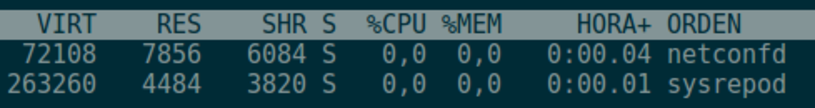
\includegraphics[scale=0.80]{Figures/consumoagentes.pdf}
		\caption{Demanda de recursos de las implementaciones analizadas.}
		\label{fig:consumoagentes}
	  \end{figure}
	\end{itemize}


	\subsubsection{Justificación de elección del agente}

	Presentado el análisis y las diferencias entre ambos proyectos, en esta sección se justificará la elección de Yuma123 como servidor que se instalará en el \textit{muxponder} de 40GB.
	\\
	
	Como se mencionó anteriormente, Sysrepo fue la primera implementación con la que se tuvo contacto y manipulación del protocolo \textit{NETCONF}. La razón por la que se optó empezar a familiarizarse con este, fue porque se encontró una gran cantidad de ejemplos y casos de uso a la hora de realizar los módulos \textit{YANG} y relacionarlos con la instrumentación y las aplicaciones Unix. Además, la instalación del proyecto en una computadora de escritorio fue sencilla (debido a la extensa documentación y las diferentes alternativas de instalación que brinda como ser \textit{dockers}, \textit{scripts} de instalación, etc).

	Sin embargo, no resultó de igual forma a la hora de realizar la compilación cruzada. La razón se debe a que Sysrepo tiene gran cantidad de dependencias como ser \textit{libyang, Google Protocol Buffers, protobuf-c, libev,} entre otros. Específicamente, se tuvo problemas para compilar la librería \textit{'protobuf-c'} para la arquitectura \textit{NIOS}, por lo que se abandonó el uso de esta herramienta. Además, como se vio anteriormente, la demanda de memoria principal y secundaria en Sysrepo excede a los recursos disponibles en el muxponder.
	\\

	En el caso de Yuma123 se logró compilar e instalar de manera correcta todas las librerías requeridas. Además, se realizaron scripts que facilitan dicha tarea para las siguientes arquitecturas: \textit{ARM, NIOS y \texttt{x86\_64}}. Cabe destacar que si bien los recursos que demanda Yuma123 son menores frente a Sysrepo, los mismos siguen siendo excesivos para el muxponder. Por lo tanto, se realizaron optimizaciones en la compilación del proyecto. Por ejemplo, se ha omitido la compilación de la librería \textit{SSH}, ya que el \textit{muxponder} ya la integra. Además, el proyecto incorpora una gran cantidad de módulos \textit{YANG} a modo de ejemplo, estos no son necesarios para el funcionamiento del mismo, por lo que también fueron omitidos. Por último, se destaca la herramienta yangdump brindada por Yuma123, la cual facilita de forma significativa el desarrollo de las librerías \textit{SIL} en \textit{C}.
	\\

	De esta forma, el factor determinante a la hora de elegir entre las distintas implementaciones \textit{NETCONF} fue tener en cuenta las limitaciones técnicas del equipo, siendo Yuma123 el agente que mejor se adaptó a las mismas. 
